%%% дбоощк жбкм ртедуфбчмсеф ртйнет йурпмшъпчбойс рблефб pazh2col
%%% дмс жптнбфйтпчбойс уфбфшй ч жптнбфе "рйуен ч буфтпопнйюеулйк цхтобм"
%%% у йурпмшъпчбоен лйтйммйюеулпк лпдйтпчлй KOI8-R.
%%% бЧФПТ: бМЕЛУБОДТ рПФЕИЙО, жфй ЙН. б.ж. йПЖЖЕ, 2023.
%%% ртедпуфбчмсефус дмс учпвпдопзп йурпмшъпчбойс: Creative Commons Zero (уу0).

%%% пРГЙС koi8-r РТЙНЕОЙНБ РТЙ ЙУРПМШЪПЧБОЙЙ ЛПДЙТПЧЛЙ KOI8-R.
%%% пРГЙС utt8 РТЙНЕОЙНБ РТЙ ЙУРПМШЪПЧБОЙЙ ЛПДЙТПЧЛЙ UTF8.
\documentclass[koi8-r]{pazh2col}
% \documentclass[utf8]{pazh2col}

%%% дБМЕЕ НПЦОП РПДЗТХЪЙФШ ДПРПМОЙФЕМШОЩЕ РБЛЕФЩ.
%%% оБРТЙНЕТ, РБЛЕФ graphicx ЙУРПМШЪХЕФУС ДМС ЧУФБЧЛЙ Ч ФЕЛУФ ТЙУХОЛПЧ:
\usepackage{graphicx}
		\usepackage{amsmath,amssymb,amsbsy} 

		\def\mprp{\mbox{\tiny $\bot$}}
		\def\mprl{\mbox{\tiny $\|$}}
		\def\th{\mbox{th}}
		\graphicspath{{Pics/}}
		\def\beq{\begin{eqnarray}}
		\def\eeq{\end{eqnarray}}
		\def\ee{\varepsilon}
		\def\lm{\lambda}
		\def\ff{\Lambda}
		\def\tff{\widetilde \Lambda}
		\def\1{1 \to 1 \, 2}
		\def\2{1 \to 2 \, 2}
		
		
		\def\beq{\begin{eqnarray}}
		\def\eeq{\end{eqnarray}}
		\def\ee{\varepsilon}
		\def\lm{\lambda}
				
		
		\newcommand{\ii}{\mathrm{i}}
		\newcommand{\dd}{\mathrm{d}}
		\newcommand{\eee}{\mathrm{e}} 

\begin{document}


\authors[тХНСОГЕЧ Й ДТ.]{
  \nextauth[rda@uniyar.ac.ru]{д. б. тХНСОГЕЧ}{1},
  \nextauth{ф.б. рХИПЧ}{1},
  \nextauth{н.ч. юЙУФСЛПЧ}{1}
}


\titles[чМЙСОЙЕ ЧОЕЫОЕК БЛФЙЧОПК УТЕДЩ]
{чМЙСОЙЕ ЧОЕЫОЕК БЛФЙЧОПК УТЕДЩ ОБ РТПГЕУУ ДЧПКОПЗП ЛПНРФПОПЧУЛПЗП ТБУУЕСОЙС}


\affiliations{
\nextaffil{сТПУМБЧУЛЙК ЗПУХДБТУФЧЕООЩК ХОЙЧЕТУЙФЕФ ЙН. р.з. дЕНЙДПЧБ, сТПУМБЧМШ,  тПУУЙС}
}


\wideabstract{
тБУУНПФТЕО РТПГЕУУ ДЧПКОПЗП ЛПНРФПОПЧУЛПЗП ТБУУЕСОЙС, $e \gamma \to e \gamma \gamma$, Ч РТЙУХФУФЧЙЙ 
УЙМШОП ЪБНБЗОЙЮЕООПК, ИПМПДОПК ЬМЕЛФТПООПК РМБЪНЩ. рПМХЮЕОБ БНРМЙФХДБ РТПГЕУУБ Й 
ОБКДЕОЩ РТБЧЙМБ ПФВПТБ РП РПМСТЙЪБГЙСН ЖПФПОПЧ. 
рПЛБЪБОП, ЮФП Ч ФБЛПК РМБЪНЕ РТПГЕУУ  ДЧПКОПЗП ЛПНРФПОПЧУЛПЗП ТБУУЕСОЙС ВХДЕФ 
ЬЖЖЕЛФЙЧОЩН НЕИБОЙЪНПН РТПЙЪЧПДУФЧБ РПМСТЙЪПЧБООЩИ ЖПФПОПЧ.

\keywords{ОЕКФТПООЩЕ ЪЧЕЪДЩ, УЙМШОПЕ НБЗОЙФОПЕ РПМЕ.}

\doi{}
} 

%=========================================================

\section{чЧЕДЕОЙЕ}
\label{introduction}

ч ОБУФПСЭЕЕ ЧТЕНС ВПМШЫПК ЙОФЕТЕУ РТЕДУФБЧМСАФ БУФТПЖЙЪЙЮЕУЛЙЕ ПВЯЕЛФЩ У НБУЫФБВБНЙ ЧЕМЙЮЙО 
НБЗОЙФОПЗП РПМС РПТСДЛБ ЙМЙ ЧЩЫЕ ЕЗП ЛТЙФЙЮЕУЛПЗП ЪОБЮЕОЙС $B_e = m^2/e \simeq 4.41\times10^{13}$ зУ -- 
ТБДЙПРХМШУБТЩ Й НБЗОЙФБТЩ~(пМБХЪЕО Й лБУРЙ, 2014). 
\footnote{йУРПМШЪХЕФУС ЕУФЕУФЧЕООБС УЙУФЕНБ ЕДЙОЙГ, ЗДЕ $c = \hbar = k_{\rm{B}} = 1$, $m$ -- НБУУБ ЬМЕЛФТПОБ,  
$e$ -- ЬМЕНЕОФБТОЩК ЪБТСД, $\alpha$ -- РПУФПСООБС ФПОЛПК УФТХЛФХТЩ.} 
 пДОПК ЙЪ РТЙОГЙРЙБМШОЩИ РТПВМЕН Ч ЖЙЪЙЛЕ УЙМШОП ЪБНБЗОЙЮЕООЩИ ОЕКФТПООЩИ ЪЧЕЪД СЧМСЕФУС ПРЙУБОЙЕ 
ПУПВЕООПУФЕК ОБВМАДБЕНЩИ УРЕЛФТПЧ Ч ПВМБУФЙ ТЕОФЗЕОПЧУЛЙИ Й ЗБННБ ЮБУФПФ, ПВХУМПЧМЕООЩИ, РП-ЧЙДЙНПНХ, 
ЧМЙСОЙЕН ТБУУЕСОЙС Й РПЗМПЭЕОЙС ЖПФПОПЧ Ч РТПГЕУУЕ РЕТЕОПУБ ЙЪМХЮЕОЙС Ч УЙМШОП ЪБНБЗОЙЮЕООПК РМБЪНЕ. 
 иПТПЫП ЙЪЧЕУФОП (УН., ОБРТЙНЕТ,~уХМЕКНБОПЧ Й чЕТОЕТ, 2007), ЮФП ЛПНРФПОПЧУЛПЕ ТБУУЕСОЙЕ, 
$e \gamma \to e \gamma$, СЧМСЕФУС ПУОПЧОЩН РТПГЕУУПН, 
ЛПФПТЩК ХЮЙФЩЧБЕФУС РТЙ ТЕЫЕОЙЙ ЪБДБЮЙ РЕТЕОПУБ ЙЪМХЮЕОЙС. пДОБЛП, ПВЭЕЕ ЮЙУМП ЖПФПОПЧ Ч РТПГЕУУЕ 
ТБУУЕСОЙС ОЕ НЕОСЕФУС. рТЕДЩДХЭЙЕ ЙУУМЕДПЧБОЙС~(юЙУФСЛПЧ Й ДТ., 2012, юЙУФСЛПЧ Й ДТ., 2016) 
РТПВМЕНЩ РЕТЕОПУБ ЙЪМХЮЕОЙС РПЛБЪБМЙ, ЮФП ТЕБЛГЙС 
ТБУЭЕРМЕОЙС ЖПФПОБ, $\gamma \to \gamma \gamma$, НПЦЕФ ЙЗТБФШ ЧБЦОХА ТПМШ ЛБЛ НЕИБОЙЪН РТПЙЪЧПДУФЧБ 
ЖПФПОПЧ. у ДТХЗПК УФПТПОЩ, ЛБЛ ВЩМП РПЛБЪБОП Ч~(юЙУФСЛПЧ Й ДТ., 2012) Ч ПВМБУФЙ ЬОЕТЗЙК ЖПФПОПЧ $\omega \ll m$ 
ОЕЛПФПТЩЕ ЛБОБМЩ ТБУЭЕРМЕОЙС ПЛБЪЩЧБАФУС ЛЙОЕНБФЙЮЕУЛЙ ЪБЛТЩФЩНЙ. рПЬФПНХ ЧПЪОЙЛБЕФ ОЕПВИПДЙНПУФШ 
ТБУУНПФТЕФШ БМШФЕТОБФЙЧОЩЕ НЕИБОЙЪНЩ ЙЪНЕОЕОЙС ЮЙУМБ ЖПФПОПЧ. ч УЙМШОП ЪБНБЗОЙЮЕООПК РМБЪНЕ ПДОЙН 
ЙЪ ФБЛЙИ НЕИБОЙЪНПЧ СЧМСЕФУС ФБЛ ОБЪЩЧБЕНПЕ ДЧПКОПЕ ЛПНРФПОПЧУЛПЕ ТБУУЕСОЙЕ, 
$e \gamma \to e \gamma \gamma$.  
 оБУЛПМШЛП ОБН ЙЪЧЕУФОП, РТПГЕУУ $e \gamma \to e \gamma \gamma$ ТБОЕЕ ТБУУНБФТЙЧБМУС ФПМШЛП 
Ч РМБЪНЕ ВЕЪ НБЗОЙФОПЗП РПМС~(мБКФНБО, 1981, лЕМШОЕТ Й ыЙИПЧГЕЧБ, 1984). ч ПВЭЕН УМХЮБЕ 
РТПЙЪЧПМШОП ЪБНБЗОЙЮЕООПК РМБЪНЩ БОБМЙЪ ЛПЬЖЖЙГЙЕОФБ РПЗМПЭЕОЙС ЖПФПОБ Ч РТПГЕУУЕ 
ДЧПКОПЗП ЛПНРФПОПЧУЛПЗП ТБУУЕСОЙС РТЕДУФБЧМСЕФ ДПУФБФПЮОП ЗТПНПЪДЛХА ЪБДБЮХ. пДОБЛП, ДМС ОЕТЕМСФЙЧЙУФУЛПК 
ЪБНБЗОЙЮЕООПК РМБЪНЩ У ФЕНРЕТБФХТПК $T \ll m$ ($\mu =0$ -- ИЙНЙЮЕУЛЙК РПФЕОГЙБМ ЬМЕЛФТПОПЧ), 
ИБТБЛФЕТОПК ДМС НБЗОЙФПУЖЕТЩ ОЕКФТПООЩИ ЪЧЕЪД, ДБЦЕ РТЙ РПМСИ $B \sim 10^{12}$ зУ ЬМЕЛФТПОЩ ВХДХФ ЪБОЙНБФШ 
РТЕЙНХЭЕУФЧЕООП ПУОПЧОПК ХТПЧЕОШ мБОДБХ, ЮФП ЪОБЮЙФЕМШОП ХРТПЭБЕФ ЧЩЮЙУМЕОЙС. ч ОБУФПСЭЕК ТБВПФЕ 
НЩ ТБУУНБФТЙЧБЕН РТПГЕУУ $e \gamma \to e \gamma \gamma$ Ч УЙМШОП ЪБНБЗОЙЮЕООПК ОЕТЕМСФЙЧЙУФУЛПК 
РМБЪНЕ У ХЮЕФПН ЙЪНЕОЕОЙС ДЙУРЕТУЙПООЩИ Й РПМСТЙЪБГЙПООЩИ УЧПКУФЧ ЖПФПОПЧ.  


%------------------------------------------------------
\section{дЙУРЕТУЙПООЩЕ УЧПКУФЧБ ЖПФПОБ Ч ЪБНБЗОЙЮЕООПК УТЕДЕ}

тБУРТПУФТБОЕОЙЕ ЬМЕЛФТПНБЗОЙФОПЗП ЙЪМХЮЕОЙС Ч МАВПК БЛФЙЧОПК УТЕДЕ ХДПВОП 
ПРЙУЩЧБФШ Ч ФЕТНЙОБИ ОПТНБМШОЩИ (УПВУФЧЕООЩИ) НПД. ч УЧПА ПЮЕТЕДШ,  
РПМСТЙЪБГЙПООЩЕ Й ДЙУРЕТУЙПООЩЕ УЧПКУФЧБ ОПТНБМШОЩИ НПД УЧСЪБОЩ У 
УПВУФЧЕООЩНЙ ЧЕЛФПТБНЙ $r_{\alpha}^{(\lambda)}$ Й УПВУФЧЕООЩНЙ ЪОБЮЕОЙСНЙ 
${\cal P}^{(\lambda)}$ РПМСТЙЪБГЙПООПЗП 
ПРЕТБФПТБ ЖПФПОБ ${\cal P}_{\alpha \beta}$ УППФЧЕФУФЧЕООП. дМС ДБМШОЕКЫЕЗП БОБМЙЪБ ЬФЙИ УЧПКУФЧ ХДПВОП ТБЪМПЦЙФШ 
ФЕОЪПТ ${\cal P}_{\alpha \beta}$ РП ВБЪЙУХ ЙЪ  
4-ЧЕЛФПТПЧ, РПУФТПЕООЩИ ЙЪ ПВЕЪТБЪНЕТЕООПЗП ФЕОЪПТБ ЬМЕЛФТПНБЗОЙФОПЗП 
РПМС Й 4-ЧЕЛФПТБ ЙНРХМШУБ ЖПФПОБ $q_\alpha$:
%
\beq
\label{eq:basis}
b_{\mu}^{(1)} = (\varphi q)_\mu, \qquad
 b_{\mu}^{(2)} = (\tilde \varphi q)_\mu, 
\\
\nonumber
b_{\mu}^{(3)} = q^2 \, (\varphi \varphi q)_\mu - q_\mu \, q^2_{\mbox{\tiny $\bot$}}, 
\qquad b_{\mu}^{(4)} = q_\mu, 
\eeq 

\noindent СЧМСАЭЙИУС УПВУФЧЕООЩНЙ ЧЕЛФПТБНЙ РПМСТЙЪБГЙПООПЗП ПРЕТБФПТБ Ч РПУФПСООПН 
ПДОПТПДОПН НБЗОЙФОПН РПМЕ. рТЙ ЬФПН $(b^{(1)} b^{*(1)}) = -q^2_{\mprp}$, 
$(b^{(2)} b^{*(2)}) = -q^2_{\mprl}$, $(b^{(3)} b^{*(3)}) = -q^2 q^2_{\mprl} 
q^2_{\mprp}$, $(b^{(4)} b^{*(4)}) = q^2$. 

йНЕЕН:  
%
%ч ЬФПН ВБЪЙУЕ ВХДЕН ЙНЕФШ УМЕДХАЭЕЕ ТБЪМПЦЕОЙЕ ${\cal P}_{\alpha \beta}$  РП УПВУФЧЕООЩН ЧЕЛФПТБН 
%$r_{\alpha}^{(\lambda)}$ Ч ЪБНБЗОЙЮЕООПК РМБЪНЕ У УППФЧЕФУФЧХАЭЙНЙ УПВУФЧЕООЩНЙ 
%ЪОБЮЕОЙСНЙ $\varkappa^{(\lambda)}$~\cite{Rojas1979r,Rojas1982,Shabad:1988,MRCh:2014}:
%
\beq
\label{eq:Pab10}
{\cal P}_{\alpha \beta} = \sum_{\lambda = 1}^{3} 
 {\cal P}^{(\lambda)} \, \frac{r_{\alpha}^{(\lambda)} 
(r_{\beta}^{(\lambda)})^{*}}{(r^{(\lambda)})^2} \, , \quad 
r_{\beta}^{(\lambda)} = \sum\limits_{i = 1}^{3} A_i^{(\lambda)} \, b_{\beta}^{(i)} \, , 
\eeq
\noindent ЗДЕ  $A_i^{(\lambda)}$ ОЕЛПФПТЩЕ ЛПНРМЕЛУОЩЕ ЛПЬЖЖЙГЙЕОФЩ.

ъДЕУШ  ЮЕФЩТЕИНЕТОЩЕ ЧЕЛФПТЩ У ЙОДЕЛУБНЙ $\bot$ Й $\parallel$ ПФОПУСФУС
УППФЧЕФУФЧЕООП Л РПДРТПУФТБОУФЧБН еЧЛМЙДБ $\{1, 2\}$ Й нЙОЛПЧУЛПЗП $\{0, 3\}$ УППФЧЕФУФЧЕООП 
Ч УЙУФЕНЕ ПФУЮЕФБ, ЗДЕ НБЗОЙФОПЕ РПМЕ ОБРТБЧМЕОП ЧДПМШ ФТЕФШЕК ПУЙ;
$(ab)_{\mprp} = (a \varphi \varphi b) = a_\alpha \varphi_{\alpha}^{\, \rho} \varphi_{\rho \beta} b_\beta$, 
$(ab)_{\mprl} = (a \tilde \varphi \tilde \varphi b) = 
a_\alpha \tilde \varphi_{\alpha}^{\, \rho} 
\tilde \varphi_{\rho \beta} b_\beta$.  $\varphi_{\alpha \beta} =  F_{\alpha
	\beta} /B$  Й
${\tilde \varphi}_{\alpha \beta} = \frac{1}{2} \varepsilon_{\alpha \beta
	\mu \nu} \varphi_{\mu \nu}$ -- ВЕЪТБЪНЕТОЩК ФЕОЪПТ ЬМЕЛФТПНБЗОЙФОПЗП РПМС 
Й ДХБМШОЩК ФЕОЪПТ  УППФЧЕФУФЧЕООП, $\beta = eB$, $q^{\mu} = (\omega, {\bf k})$. 

тЕЫЕОЙЕ ЬФПК ЪБДБЮЙ ДМС РТПЙЪЧПМШОП ЪБНБЗОЙЮЕООПК РМБЪНЩ РТЕДУФБЧМСЕФ ЪОБЮЙФЕМШОЩЕ ЧЩЮЙУМЙФЕМШОЩЕ 
ФТХДОПУФЙ Й ТБОЕЕ ТЕЫБМБУШ ДМС УМХЮБС, ЛПЗДБ МЙДЙТХАЭЙНЙ СЧМСАФУС РБТБНЕФТЩ РМБЪНЩ ФБЛЙЕ, ЛБЛ 
ФЕНРЕТБФХТБ, ИЙНЙЮЕУЛЙК РПФЕОГЙБМ Й Ф.Д. (УН., ОБРТЙНЕТ, рПФЕИЙО Й ДТ., 2004). 
 у  ДТХЗПК УФПТПОЩ, Ч УМХЮБЕ УЙМШОП ЪБНБЗОЙЮЕООПК РМБЪНЩ, ЛПЗДБ НБЗОЙФОПЕ РПМЕ СЧМСЕФУС 
ОБЙВПМШЫЙН  РБТБНЕФТПН ЪБДБЮЙ,
$\beta \gg m^2,\, \mu^2, \, T^2, \, q^2_{\mprl}$, Ч ПВМБУФЙ $q^2_{\mprl} \ll (m+\sqrt{m^2+2 \beta})^2$, 
ЙУРПМШЪХС 
ТЕЪХМШФБФЩ ТБВПФ~(рЕТЕУ тПИБУ, 1979, нЙИЕЕЧ Й ДТ., 2014)
%~\cite{Rojas1979,Rojas1982,Rojas1979r,Shabad:1988} 
ДМС ${\cal P}_{\alpha \beta}$, НПЦОП РПМХЮЙФШ УМЕДХАЭЕЕ ТБЪМПЦЕОЙЕ РП 
ПВТБФОЩН УФЕРЕОСН НБЗОЙФОПЗП РПМС:
%
\beq
\nonumber
&&{\cal P}_{\alpha \beta}  
 \simeq 
 - \frac{2\alpha}{\pi} \; \beta \, {\cal D} \, 
\frac{(\tilde \varphi q)_\alpha (\tilde \varphi q)_\beta}{q^2_{\mprl}} 
+ 
\frac{\alpha}{3\pi}\; (\varphi q)_\alpha (\varphi q)_\beta +
\\
\nonumber
&&+\frac{\ii \alpha}{\pi} \, \Delta N \, \left [
\varphi_{\alpha \beta} \, (qu) + (q\varphi)_{\alpha} u_{\beta} - 
(q\varphi)_{\beta} u_{\alpha} \right ]  +
\\
\label{eq:Pab1}
&& + \frac{\alpha}{3\pi} \, {\cal V} \, \left (q^2 \, g_{\alpha \beta} - 
q_{\alpha} \, q_{\beta} \right )  + 
O \left (\frac{1}{\beta} \right) \, , 
\eeq  
\noindent ЗДЕ 
%
\beq
\label{eq:PabD}
{\cal D} = - {\cal J} (q_{\mprl})  - 
H \left (\frac{q^2_{\mprl}}{4m^2} \right)  \, , 
\eeq
%
\beq
\label{eq:PabJ}
{\cal J} (q_{\mprl}) = 2q^2_{\mprl} \, m^2 \, \int\limits_{-\infty}^{\infty}  \frac{\dd p_z}{E} \, 
\frac{f_{-}(p) + f_{+}(p)}{q_{\mprl}^4 - 4(pq)^2_{\mprl}} \, , 
\eeq
%
\beq
\label{eq:fermidist}
&&f_{\pm}(p) = \frac{1}{1+\exp{[((pu)_{\mprl} \pm \mu)/T]}} \, , 
\\ [3mm]
\nonumber
&&(pu)_{\mprl} = E u_0 - p_z u_z \, , \quad E=\sqrt{p_z^2+m^2} \, .
\eeq
\noindent ъДЕУШ ЧЕТИОЙК ЪОБЛ УППФЧЕФУФЧХЕФ ЬМЕЛФТПООПК, Б ОЙЦОЙК -- РПЪЙФТПООПК ЛПНРПОЕОФБН РМБЪНЩ.

%
\beq
\label{eq:H0}
\nonumber
%\nonumber
&&H(z)=\frac{1}{\sqrt{z(1 - z)}} \, \arctg \sqrt{\frac{z}{1 - z}} - 1,
\\
\label{eq:H1}
 &&0 \leqslant z \leqslant 1,
%H(z) &=& - \frac{1}{2\sqrt{z(z-1)}}
%\ln  \frac{\sqrt{z} + \sqrt{z-1}}{\sqrt{z} - \sqrt{z-1}}  - 1 + 
%\\[3mm]
%\nonumber
%&+& \frac{i\pi}{2\sqrt{z(z-1)}}, \quad z > 1, 
\eeq
%
\beq
\nonumber
\Delta N &=& \int\limits_{-\infty}^{\infty}  \frac{\dd p_z}{E} 
\, (pu)_{\mprl} \, \left [f_{-}(p) - f_{+}(p) \right] = 
\\
\label{eq:PabA}
&=& \frac{(2 \pi)^2}{\beta} \, (n_{e} - n_{e^+}) \, , 
%\\
%\nonumber 
%&&f((pu),\mu) = \left [\exp{((pu)-\mu)/T} + 1 \right ]^{-1}  \, , \quad   E=\sqrt{p^2+m^2} \, , 
\eeq
\noindent $n_{e}$ $(n_{e^+})$ -- ЛПОГЕОФТБГЙС ЬМЕЛФТПОПЧ (РПЪЙФТПОПЧ) РМБЪНЩ, 
%
\beq
\label{eq:Lambda}
{\cal V} &=& \ln{(B/B_e)} - 1.792 + 
\\
\nonumber
&+&
\frac{3}{2} \, \int\limits_0^1 \dd x \, (1-x^2) \, 
\ln{\left [1- \frac{q^2}{4m^2} \, (1-x^2) \right ]} \, .
\eeq

ч УЙУФЕНЕ РПЛПС РМБЪНЩ $(pu)_{\mprl} = E$ Й ДМС  
  ТБЪМПЦЕОЙС УПВУФЧЕООЩИ ЧЕЛФПТПЧ $r^{(\lambda)}_{\alpha}$ РП ПВТБФОЩН УФЕРЕОСН 
РПМС  РПМХЮЙН:  
%
\beq
\label{eq:r13}
&&r^{(1,3)}_{\alpha} = \left [\mp \sqrt{q^4_{\mprp} + 
(6 \Delta N \, \omega)^2\, \frac{q^2}{q_{\mprl}^2}}  - q^2_{\mprp} \right ]\, 
b^{(1)}_{\alpha} - 
\\
\nonumber
&&-
\ii \, \frac{6 \Delta N \, \omega}{q_{\mprl}^2} \,  b^{(3)}_{\alpha} +
 \ii \,\frac{\Delta N \, k_z \, q^2_{\mprp}}{2\beta \, {\cal D} \, q^2_{\mprl}}\, 
\times
\\
\nonumber 
&& \times
\left [\pm \sqrt{q^4_{\mprp} + 
(6 \Delta N \, \omega)^2\, \frac{q^2}{q_{\mprl}^2}} + q^2_{\mprp} \right ]\; b^{(2)}_{\alpha} + 
O \left (\frac{1}{\beta^2} \right) \, ,
\eeq
%
\beq
\label{eq:r2}
r^{(2)}_{\alpha} =  b^{(2)}_{\alpha} - 
\ii \, \frac{\Delta N  \, k_z }{2\beta \, {\cal D}} \, b^{(1)}_{\alpha} + 
O \left (\frac{1}{\beta^2} \right)  \, .
\eeq


уППФЧЕФУФЧХАЭЙЕ УПВУФЧЕООЩЕ ЪОБЮЕОЙС ${\cal P}^{(\lambda)}$ Ч РТЙВМЙЦЕОЙЙ 
$O(1/\beta)$  ЪБРЙЫХФУС УМЕДХАЭЙН ПВТБЪПН:
%
\beq
\label{eq:kappa13}
&&{\cal P}^{(1,3)} = \frac{\alpha}{3\pi} \, q^2 \, {\cal V} + 
\\
\nonumber
&&+
\frac{\alpha}{6\pi} \, \left [ 
 \mp \sqrt{q^4_{\mprp} + 
(6 \Delta N \, \omega)^2\, \frac{q^2}{q_{\mprl}^2}}  - q^2_{\mprp} \right ]  
+ O \left (\frac{1}{\beta} \right)  \, ,
\eeq
%
\beq
\label{eq:kappa2}
{\cal P}^{(2)} = \frac{\alpha}{3\pi} \, q^2 \, {\cal V} + \frac{2 \alpha}{\pi} \, \beta \, {\cal D}  + 
 O \left (\frac{1}{\beta} \right) \, .
\eeq

ч  УМХЮБЕ ЪБТСДПЧП УЙННЕФТЙЮОПК РМБЪНЩ $\Delta N = 0$, 
УПВУФЧЕООЩЕ ЧЕЛФПТЩ~(\ref{eq:r13}) -- (\ref{eq:r2}) Й 
УПВУФЧЕООЩЕ ЪОБЮЕОЙС~(\ref{eq:kappa13}) -- (\ref{eq:kappa2}) РТЙНХФ ЧЙД:
%
\beq
\label{eq:r130}
r^{(1)}_{\alpha} =  -2 q^2_{\mprp} \, b^{(1)}_{\alpha}  + O \left (\frac{1}{\beta^2} \right) \, ,
\quad   r^{(3)}_{\alpha} =  O \left (\frac{1}{\beta^2} \right) \, ,
\eeq
%
\beq
\label{eq:r20}
r^{(2)}_{\alpha} =  b^{(2)}_{\alpha}  + O \left (\frac{1}{\beta^2} \right)  \, .
\eeq


%
\beq
\label{eq:kappa10}
&&{\cal P}^{(1)} = \frac{\alpha}{3\pi} \, q^2 \, {\cal V} - \frac{\alpha}{3\pi} \, 
q^2_{\mprp} + O \left (\frac{1}{\beta} \right)  \, ,
\\[3mm]
\label{eq:kappa30}
&&{\cal P}^{(3)} = \frac{\alpha}{3\pi} \, q^2 \, {\cal V} + O \left (\frac{1}{\beta} \right)  \, ,
\eeq
%
\noindent Б УПВУФЧЕООПЕ ЪОБЮЕОЙЕ  ${\cal P}^{(2)}$ ПРТЕДЕМСЕФУС ЖПТНХМПК~(\ref{eq:kappa2}).


  уМЕДХЕФ ПФНЕФЙФШ, ЮФП РПМХЮЕООЩЕ УПВУФЧЕООЩЕ ЧЕЛФПТЩ~(\ref{eq:r130}) Й~(\ref{eq:r20}) РПМСТЙЪБГЙПООПЗП 
ПРЕТБФПТБ Ч ЪБТСДПЧП УЙННЕФТЙЮОПК РМБЪНЕ ОЕ СЧМСАФУС ОПТНЙТПЧБООЩНЙ. рПЬФПНХ ДМС ПРЙУБОЙС 
РПМСТЙЪБГЙПООЩИ УПУФПСОЙК ЖПФПОПЧ Ч ФБЛПК РМБЪНЕ ХДПВОП ЧЧЕУФЙ ОПТНЙТПЧБООЩЕ ЧЕЛФПТЩ
%
\beq
\label{eq:epsilon}
&&\varepsilon_\alpha^{(1)}(q) = \frac{r^{(1)}_{\alpha}}{\sqrt{|(r^{(1)} r^{*(1)})|}} = 
\frac{(q \varphi)_\alpha}{\sqrt{q_{\mprp}^2}},
\\
\nonumber
&&\varepsilon_\alpha^{(2)}(q) = \frac{r^{(2)}_{\alpha}}{\sqrt{|(r^{(2)} r^{*(2)})|}} = 
\frac{(q \tilde \varphi)_\alpha}{\sqrt{q_{\mprl}^2}}.
\eeq
%
\noindent ъДЕУШ УЙНЧПМЩ 1 Й 2 УППФЧЕФУФЧХАФ  
$X$ - Й $O$ -  НПДБН ПВЩЮОП ЙУРПМШЪХЕНЩН Ч МЙФЕТБФХТЕ~(УН., ОБРТЙНЕТ, нХЫФХЛПЧ Й ДТ., 2016).  

 оЕФТХДОП ЧЙДЕФШ, ЮФП ЧЧЕДЕООЩЕ ФБЛЙН ПВТБЪПН РПМСТЙЪБГЙПООЩЕ УПУФПСОЙС Ч ЪБТСДПЧП УЙННЕФТЙЮОПК 
РМБЪНЕ,  У ФПЮОПУФША ДП $O(1/\beta)$ Й $O(\alpha^2)$, ЙНЕАФ ФПФ ЦЕ ЧЙД, ЮФП Й Ч  ЪБНБЗОЙЮЕООПН 
ЧБЛХХНЕ~\footnote{рПД ФЕТНЙОПН <<ЪБНБЗОЙЮЕООЩК ЧБЛХХН>>  
РПОЙНБЕФУС НБЗОЙФОПЕ РПМЕ ВЕЪ РМБЪНЩ.}. дБООЩК ЧЩЧПД УПЗМБУХЕФУС У ТЕЪХМШФБФБНЙ ТБВПФЩ 
(ыБВБД, 1988), Б Ч РТЕДЕМЕ $\omega \ll m$, РПУМЕ ОБДМЕЦБЭЙИ РТЕПВТБЪПЧБОЙК (ЧЩДЕМЕОЙЕ РТПУФТБОУФЧЕООПК 
ЮБУФЙ ЧЕЛФПТБ $\varepsilon^{(2)}_\alpha$ Й РЕТЕИПД Л УЙУФЕНЕ ЛППТДЙОБФ, ЗДЕ ЧЕЛФПТ ЙНРХМШУБ ЖПФПОБ 
ОБРТБЧМЕО ЧДПМШ ПУЙ $z$), У ТЕЪХМШФБФБНЙ ТБВПФЩ (рПФЕИЙО Й ДТ., 2004). 

лТПНЕ ФПЗП, Ч РТЙВМЙЦЕОЙЙ $O(1/\beta)$ ЪБЛПО ДЙУРЕТУЙЙ ЖПФПОБ НПДЩ 1 РТБЛФЙЮЕУЛЙ ОЕ ПФМЙЮБЕФУС 
ПФ ЧБЛХХНОПЗП, $q^2 \simeq 0$. дЕКУФЧЙФЕМШОП, ЙЪ ХТБЧОЕОЙС ДЙУРЕТУЙЙ ДМС ЬФПК НПДЩ
%
\beq
q^2 - {\cal P}^{(1)} = 0 \, 
\label{disper1}
\eeq
\noindent Й ЖПТНХМЩ~(\ref{eq:kappa10}) УМЕДХЕФ, ЮФП 
%
\beq
q_{\mprl}^2 = \left (1- \frac{\alpha}{3\pi} \frac{1}{1-\frac{\alpha}{3\pi} \cal V} \right) \, q_{\mprp}^2  
\simeq q_{\mprp}^2 \left (1- \frac{\alpha}{3\pi} \right)\, , 
\label{disper12}
\eeq
\noindent ФБЛ, ЮФП  $q^2 \simeq 0$, 
ПУФБЧБСУШ РТЙ ЬФПН ПФТЙГБФЕМШОЩН. лТПНЕ ФПЗП, ЙЪ ЖПТНХМЩ~(\ref{eq:kappa10}) УМЕДХЕФ, ЮФП Ч 
ПВМБУФЙ $q^2_{\mprl} \ll (m+\sqrt{m^2+2 \beta})^2$ Х УПВУФЧЕООПЗП ЪОБЮЕОЙС РПМСТЙЪБГЙПООПЗП 
ПРЕТБФПТБ ЖПФПОБ, УППФЧЕФУФЧХАЭЕЗП НПДЕ 1 ПФУХФУФЧХЕФ НОЙНБС ЮБУФШ~\footnote{уФТПЗП ЗПЧПТС, НОЙНБС ЮБУФШ 
ПЛБЪЩЧБЕФУС УЙМШОП РПДБЧМЕООПК,  РП УТБЧОЕОЙА У ТЕБМШОПК ЮБУФША, ФБЛ, ЮФП ФБЛПК ЖПФПО ВХДЕФ ЛЧБЪЙУФБВЙМШОЩН 
(УН., ОБРТЙНЕТ, сТЛПЧ Й ДТ, 2022)}, ЮФП РТЙЧПДЙФ Л ОЕЧПЪНПЦОПУФЙ 
ТПЦДЕОЙС $e^+e^-$ РБТЩ  ФБЛЙН ЖПФПОПН Ч ЬФПК ПВМБУФЙ.  

 
у ДТХЗПК УФПТПОЩ, ДЙУРЕТУЙПООЩЕ УЧПКУФЧБ ЖПФПОБ НПДЩ 2  РТЕФЕТРЕЧБАФ УХЭЕУФЧЕООЩЕ ЙЪНЕОЕОЙС ДБЦЕ 
РП УТБЧОЕОЙА У ЪБНБЗОЙЮЕООЩН ЧБЛХХНПН Й, УМЕДПЧБФЕМШОП, ВХДХФ ПЛБЪЩЧБФШ ДПРПМОЙФЕМШОПЕ ЧМЙСОЙЕ 
ОБ ЛЙОЕНБФЙЛХ РТПГЕУУПЧ У 
ХЮБУФЙЕН ЖПФПОПЧ ЬФПК НПДЩ. тБУУНПФТЙН ДБООПЕ ХФЧЕТЦДЕОЙЕ ВПМЕЕ РПДТПВОП.
оБ ТЙУ.~\ref{fig:disT}  Ч ЛБЮЕУФЧЕ ЙММАУФТБГЙЙ РТЕДУФБЧМЕОЩ ЪБЛПОЩ ДЙУРЕТУЙЙ ЖПФПОБ  НПДЩ 2 ДМС УМХЮБС, ЛПЗДБ 
ЖПФПО ТБУРТПУФТБОСЕФУС РПРЕТЕЛ НБЗОЙФОПЗП РПМС, 
ЛБЛ  ТЕЫЕОЙС ХТБЧОЕОЙС
%
\beq
q^2 - {\cal P}^{(2)} = 0 \, 
\label{disper}
\eeq
\noindent  Ч ЪБНБЗОЙЮЕООПК РМБЪНЕ ДМС ТБЪМЙЮОЩИ ЪОБЮЕОЙК ФЕНРЕТБФХТ. 
лБЛ ОЕФТХДОП ЧЙДЕФШ, Ч РТПФЙЧПРПМПЦОПУФШ ЮЙУФПНХ 
НБЗОЙФОПНХ РПМА, Ч РМБЪНЕ УХЭЕУФЧХЕФ ПВМБУФШ У  $q^2 > 0$ ОЙЦЕ  ЛЙОЕНБФЙЮЕУЛПЗП  РПТПЗБ 
ТПЦДЕОЙС $e^+e^-$ РБТЩ, ПРТЕДЕМСЕНПЗП ХУМПЧЙЕН $q^2_{\mprl} = 4 m^2$.  

%%%%%%%%%%%%%%%%%%%%%%%%%%%%%%%%%%%%%%%%%%%%%%%%%%%%%%%%%
\begin{figure}
\centering
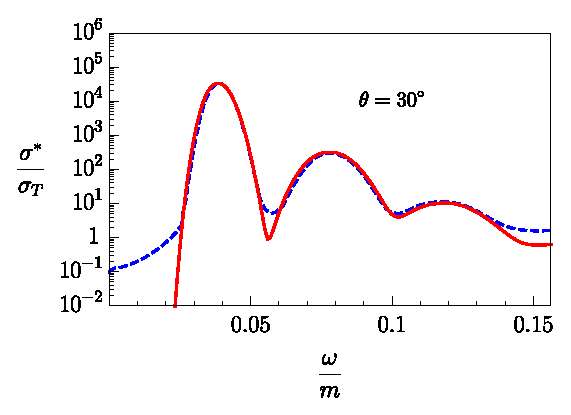
\includegraphics[width=\columnwidth]{fig2_1.eps}
\caption{ъБЛПОЩ ДЙУРЕТУЙЙ ЖПФПОБ НПДЩ 2 Ч УЙМШОПН НБЗОЙФОПН РПМЕ  $B/B_e = 200$  
Й ОЕКФТБМШОПК РМБЪНЕ ДМС ТБЪМЙЮОЩИ ЪОБЮЕОЙК ФЕНРЕТБФХТЩ:  $T = 1$ нЬч 
(ЧЕТИОСС ЛТЙЧБС), $T = 0.5$ нЬч (УТЕДОСС ЛТЙЧБС), $T = 0.25$ нЬч (ОЙЦОСС ЛТЙЧБС). 
дЙУРЕТУЙС ЖПФПОБ ВЕЪ РМБЪНЩ ПВПЪОБЮЕОБ ЫФТЙИПЧПК МЙОЙЕК. дЙБЗПОБМШОБС ЫФТЙИПЧБС 
МЙОЙС УППФЧЕФУФЧХЕФ ЧБЛХХНОПНХ ЪБЛПОХ ДЙУРЕТУЙЙ, $q^2 = 0$. 
хЗПМ  НЕЦДХ ЙНРХМШУПН ЖПФПОБ  Й ОБРТБЧМЕОЙЕН  НБЗОЙФОПЗП РПМС ТБЧЕО  $\pi/2$.
}
\label{fig:disT}
\end{figure}
%%%%%%%%%%%%%%%%%%%%%%%%%%%%%%%%%%%%%%%%%%%%%%%%%%%%%%%%%

ьФПФ ЖБЛФ УЧСЪБО  У
 РПСЧМЕОЙЕН РМБЪНЕООПК ЮБУФПФЩ Ч РТЙУХФУФЧЙЙ ТЕБМШОЩИ ЬМЕЛФТПОПЧ Й РПЪЙФТПОПЧ УТЕДЩ, 
ЛПФПТБС НПЦЕФ ВЩФШ ПРТЕДЕМЕОБ ЙЪ ХТБЧОЕОЙС

%
\begin{equation}
\omega_{pl}^2 - {\cal P}^{(2)} (\omega_{pl}, {\mathbf k} \to 0 ) = 0.
\label{eq:omegapl}
\end{equation}

ч УМХЮБЕ УЙМШОП ЪБНБЗОЙЮЕООПК, ОЕТЕМСФЙЧЙУФУЛПК РМБЪНЩ ХТБЧОЕОЙЕ~(\ref{eq:omegapl}) НПЦЕФ 
ВЩФШ ТЕЫЕОП РТЙВМЙЦЕООП. ч ТЕЪХМШФБФЕ РПМХЮЙН $\omega_{pl}^2 \simeq (8\pi \alpha n_{e})/m$, 
ЗДЕ 
%
\begin{eqnarray}
n_{e} \simeq \beta \sqrt{\frac{mT}{(2\pi)^3}}\,e^{-m/T}.
\label{eq:ne}
\end{eqnarray}
  
ч ЮБУФОПУФЙ, ДМС ЪОБЮЕОЙС ФЕНРЕТБФХТЩ $T=50$ ЛЬч Й ЧЕМЙЮЙОЩ НБЗОЙФОПЗП РПМС $B=200 B_e$  РПМХЮЙН
УМЕДХАЭХА ПГЕОЛХ: $\omega_{pl} \simeq 3$ ЛЬч, ЮФП НПЦЕФ РПЧМЙСФШ ОБ ЛЙОЕНБФЙЛХ ТБЪМЙЮОЩИ ЖПФПООЩИ РТПГЕУУПЧ.  
оБРТЙНЕТ, ДМС ПДОПК ЙЪ ПУОПЧОЩИ ТЕБЛГЙК РП РТПЙЪЧПДУФЧХ РПМСТЙЪПЧБООЩИ ЖПФПОПЧ, ЛПФПТПК СЧМСЕФУС 
РТПГЕУУ ТБУЭЕРМЕОЙС ЖПФПОБ ОБ ДЧБ ЖПФПОБ, $\gamma \to \gamma \gamma$,  ОБМЙЮЙЕ  РМБЪНЕООПК 
ЮБУФПФЩ, РТЙЧПДЙФ Л ОПЧЩН РТБЧЙМБН ПФВПТБ РП РПМСТЙЪБГЙСН: Ч ПВМБУФЙ ОЙЦЕ РПТПЗБ ТПЦДЕОЙС 
$e^+e^-$ РБТЩ, $q^2_{\mprl} = 4 m^2$  Й Ч ПВМБУФЙ $q^2 > 0$ ЛБОБМЩ ТБУЭЕРМЕОЙС, ПФЧЕЮБАЭЙЕ 
ЪБ РТПЙЪЧПДУФЧП ЖПФПОПЧ НПДЩ 2,   
$\gamma_2 \to \gamma_2 \gamma_2$, 
$\gamma_1 \to \gamma_2 \gamma_2$ Й $\gamma_1 \to \gamma_1 \gamma_2$ ПЛБЪЩЧБАФУС 
ЛЙОЕНБФЙЮЕУЛЙ ЪБЛТЩФЩНЙ. ч ЬФПК ПВМБУФЙ ТБЪТЕЫЕО ФПМШЛП ЛБОБМ $\gamma_2 \to \gamma_1 \gamma_1$ 
ПФЧЕЮБАЭЙК ЪБ РТПЙЪЧПДУФЧП ЖПФПОПЧ НПДЩ 1.  уМЕДПЧБФЕМШОП, Ч ЬФПН УМХЮБЕ МЙДЙТХАЭЙН ЛБОБМПН РП РТПЙЪЧПДУФЧХ 
ЖПФПОПЧ НПДЩ 2 ВХДЕФ 
РТПГЕУУ ДЧПКОПЗП ЛПНРФПОПЧУЛПЗП ТБУУЕСОЙС, $e \gamma_2 \to e \gamma_2 \gamma_2$.

%------------------------------------------------------
\section{ьЖЖЕЛФЙЧОПУФШ РТПЙЪЧПДУФЧБ ЖПФПОПЧ}

ч  ХУМПЧЙСИ УЙМШОП ЪБНБЗОЙЮЕООПК ОЕТЕМСФЙЧЙУФУЛПК  РМБЪНЩ $(T \ll m)$
ЛПЬЖЖЙГЙЕОФ РПЗМПЭЕОЙС ЖПФПОБ ДМС  ЛБОБМБ $e \gamma_2 \to e \gamma_2 \gamma_2$
НПЦЕФ ВЩФШ ЧЩТБЦЕО Ч 
ФЕТНЙОБИ  УЕЮЕОЙС   $W_{2 \to 22} = n_e \sigma_{2 \to 22}$:  
%
\begin{eqnarray}
\nonumber
&&d\sigma_{2 \to 22} \simeq \frac{1}{2^5 (2\pi)^5 m^2 \omega} 
 d\Omega'  d\Omega''  d \omega'' \times
\\
\label{eq:crosssec222}
&&\times \omega'' (\omega - \omega'') \mid {\cal M}_{2 \to 22}\mid^2 \, ,
\end{eqnarray}
\noindent ЗДЕ $n_e$ -- ЛПОГЕОФТБГЙС ЬМЕЛФТПОПЧ, 
%
\begin{eqnarray}
\nonumber
&&{\cal M}_{2 \to 22} \simeq -2 \,
\frac{(4 \pi \alpha)^{3/2}}{m} \; \sin{\theta} \sin{\theta'} \sin{\theta''}\times 
\\
\label{eq:amp222}
&&\times \left [ \left(2 - \frac{\omega''}{\omega} \right ) \cos{\theta'} + 
\left(1 + \frac{\omega''}{\omega} \right ) \cos{\theta''}\right ]
\end{eqnarray}
\noindent -- РБТГЙБМШОБС БНРМЙФХДБ Ч МЙДЙТХАЭЕН РТЙВМЙЦЕОЙЙ,  
$q^{\alpha} = (\omega, {\bf k})$, $q'^{\alpha} = (\omega', {\bf k}')$ Й 
$q''^{\alpha} = (\omega'', {\bf k}'')$ -- ЮЕФЩТЕИНЕТОЩЕ ЙНРХМШУЩ ОБЮБМШОПЗП Й ЛПОЕЮОЩИ ЖПФПОПЧ 
УППФЧЕФУФЧЕООП, 
$\theta$, $\theta'$ Й $\theta''$  -- ХЗМЩ НЕЦДХ ЙНРХМШУБНЙ ЖПФПОПЧ, ${\bf k}$, ${\bf k}'$  Й ${\bf k}''$ Й 
ОБРТБЧМЕОЙЕН НБЗОЙФОПЗП РПМС УППФЧЕФУФЧЕООП. 

пФНЕФЙН, ЮФП ЪБНБЗОЙЮЕООБС РМБЪНБ НПЦЕФ ПЛБЪЩЧБФШ ЧМЙСОЙЕ ЛБЛ ОБ БНРМЙФХДЩ ЛЧБОФПЧЩИ 
РТПГЕУУПЧ, ФБЛ Й ОБ ЙИ ЛЙОЕНБФЙЛХ. пДОБЛП Ч УЙМШОП ЪБНБЗОЙЮЕООПК ОЕТЕМСФЙЧЙУФУЛПК РМБЪНЕ ЕЈ 
ЧМЙСОЙЕ ОБ БНРМЙФХДХ ВХДЕФ ВПМЕЕ 
ЧЩУПЛПЗП РПТСДЛБ НБМПУФЙ РП ЛПОУФБОФЕ ЬМЕЛФТПНБЗОЙФОПЗП ЧЪБЙНПДЕКУФЧЙС Й ЙН НПЦОП РТЕОЕВТЕЮШ. рПЬФПНХ, 
ПУОПЧОПЕ ЧМЙСОЙЕ ЪБНБЗОЙЮЕООПК РМБЪНЩ  ВХДЕФ ОБ ЙЪНЕОЕОЙЕ ЛЙОЕНБФЙЛЙ РТПГЕУУБ $\gamma e \to e \gamma \gamma$ Й, 
ЛБЛ УМЕДУФЧЙЕ ОБ ЙЪНЕОЕОЙЕ ЖБЪПЧПЗП ПВЯЕНБ ТЕБЛГЙЙ.
 рТЙ ЬФПН УЕЮЕОЙЕ ТБУУЕСОЙС ДМС ТЕБЛГЙЙ 
$e \gamma_2 \to e \gamma_2 \gamma_2$ ВХДЕФ ЙНЕФШ РПТПЗ, $\omega = 2 \omega_{pl}$ (УН. ТЙУ.~\ref{fig:disT} 
Й ХТБЧОЕОЙЕ~(\ref{eq:omegapl})). рТЙЮЙОПК ЬФПЗП СЧМСЕФУС ФПФ ЖБЛФ, ЮФП Ч 
УЙМХ  ХТБЧОЕОЙС ДЙУРЕТУЙЙ~(\ref{disper}) ДМС ЖПФПОБ НПДЩ 2 У ХЮЕФПН РМБЪНЕООПК ЮБУФПФЩ, ЬМЕЛФТПНБЗОЙФОБС ЧПМОБ, 
УППФЧЕФУФЧХАЭБС ЬФПК НПДЕ, ОЕ НПЦЕФ ТБУРТПУФТБОСФШУС У ЬОЕТЗЙЕК ОЙЦЕ  $\omega_{pl}$. ьФП ЬЛЧЙЧБМЕОФОП 
РТЙПВТЕФЕОЙА ЖПФПОПН <<ЬЖЖЕЛФЙЧОПК>> НБУУЩ, УППФЧЕФУФЧХАЭЕК РМБЪНЕООПК ЮБУФПФЕ.
 у ХЮЕФПН ЬФПЗП ЪБНЕЮБОЙС, ЛЙОЕНБФЙЮЕУЛБС ПВМБУФШ РП $\omega''$  ПРТЕДЕМСЕФУС ОЕТБЧЕОУФЧПН 
$\omega_{pl} \leq \omega'' \leq \omega-\omega_{pl}$.
 рПУМЕ ЙОФЕЗТЙТПЧБОЙС~(\ref{eq:crosssec222}) РП $d \omega''$, 
РПМХЮЙН РТПУФПЕ ЧЩТБЦЕОЙЕ ДМС ДЙЖЖЕТЕОГЙБМШОПЗП УЕЮЕОЙС, ХДПВОПЕ 
ДМС ЙУРПМШЪПЧБОЙС Ч ЪБДБЮЕ РЕТЕОПУБ ЙЪМХЮЕОЙС:
%
\begin{eqnarray}
\nonumber
&&\frac{d \sigma_{2 \to 22}}{d\Omega' d\Omega''} \simeq \frac{\alpha^3 }{240 \pi^2 m^4} \; 
(\omega-2\omega_{pl}) \Theta (\omega-2\omega_{pl}) \times
\\
\nonumber
&& \times \sin^2{\theta} \sin^2{\theta'} \sin^2{\theta''} \Big [(\omega +2 \omega_{pl})(23 \cos^2{\theta'} +
\\
\nonumber
&&+ 44 \cos{\theta'} \cos{\theta''}  
+23 \cos^2{\theta''}) -
\\
\nonumber
&& -
\frac{2 \omega_{pl}^2}{\omega} 
(29 \cos^2{\theta'} + 
32 \cos{\theta'} \cos{\theta''} + 29 \cos^2{\theta''}) + 
\\
\label{eq:difcross222}
&&
+\frac{12 \omega_{pl}^3}{\omega^3} (2 \omega - \omega_{pl}) (\cos{\theta'} -\cos{\theta''})^2 \Big] \, , 
\end{eqnarray}
\noindent ЗДЕ $\Theta (x)$ -- фЬФБ-ЖХОЛГЙС. 

ч РТЙВМЙЦЕОЙЙ  ЙЪПФТПРОПЗП ТБУРТЕДЕМЕОЙС ЖПФПОПЧ ЙОФЕЗТЙТПЧБОЙЕ~(\ref{eq:crosssec222}) РП ФЕМЕУОЩН 
ХЗМБН  $d \Omega'$  Й  $d \Omega''$  ДБЕФ
%
\begin{eqnarray}
\label{eq:difcromega}
&&\frac{d \sigma_{2 \to 22}}{d\omega''} = \frac{8 \alpha^3 \sin^2{\theta}}{45  m^4} \, \omega'' 
\left(1-\frac{\omega''}{\omega} \right) \times 
\\
\nonumber
&& \times
\left [5 - 2 \frac{\omega''}{\omega} \left(1-\frac{\omega''}{\omega} \right) \right] 
\Theta (\omega-2\omega_{pl}) \times
\\
\nonumber
&&\times
\Theta (\omega - \omega_{pl} -\omega'') \Theta (\omega''-\omega_{pl})\, .
\end{eqnarray}

ч ЛБЮЕУФЧЕ РТЙМПЦЕОЙС РПМХЮЕООЩИ ТЕЪХМШФБФПЧ ТБУУНПФТЙН  ЛЙОЕФЙЮЕУЛПЕ ХТБЧОЕОЙЕ ДМС ЖХОЛГЙЙ ТБУРТЕДЕМЕОЙС 
ЖПФПОПЧ НПДЩ 2, У ХЮЕФПН ФПМШЛП РТПГЕУУБ ДЧПКОПЗП ЛПНРФПОПЧУЛПЗП ТБУУЕСОЙС, ЛПФПТПЕ  НПЦЕФ
ВЩФШ ЪБРЙУБОП Ч УМЕДХАЭЕН ЧЙДЕ (УН., ОБРТЙНЕТ, лЕМШОЕТ Й ыЙИПЧГЕЧБ, 1984):
%
\begin{eqnarray} 
\label{Kinet:Gen}
&&\frac{\partial f_{\omega,\theta}(t,z)}{\partial t} + 
\cos{\theta} \frac{\partial f_{\omega,\theta}(t,z)}{\partial z} = 
\\
\nonumber
&& = n_e \int d\sigma_{2\to 22} 
\big \{f_{\omega',\theta'}(t,z) f_{\omega'',\theta''}(t,z) \times  
\\
\nonumber
&&\times (1+f_{\omega, \theta}(t,z))-f_{\omega,\theta}(t,z) 
(1+ f_{\omega',\theta'}(t,z)) \times 
\\
\nonumber
&&\times
(1+f_{\omega'',\theta''}(t,z)) \big \} \, .
\end{eqnarray}
\noindent ъДЕУШ ХЮФЕОП, ЮФП НБЗОЙФОПЕ РПМЕ ОБРТБЧМЕОП ЧДПМШ ПУЙ $z$.

бОБМЙЪ ХТБЧОЕОЙС~(\ref{Kinet:Gen}) У ХЮЕФПН~(\ref{eq:difcromega}) Ч  МЙДЙТХАЭЕН РП $\omega_{pl}$  
РТЙВМЙЦЕОЙЙ РПЪЧПМСЕФ РПМХЮЙФШ УМЕДХАЭХА ПГЕОЛХ ЮЙУМБ 
ЖПФПОПЧ НПДЩ 2, ТПЦДБЕНЩИ Ч РТПГЕУУЕ 
$e \gamma \to e \gamma \gamma$ Ч НБЗОЙФПУЖЕТЕ УЙМШОП ЪБНБЗОЙЮЕООПК ОЕКФТПООПК ЪЧЕЪДЩ:
%
\begin{eqnarray}
\label{eq:number222}
&&\frac{d N}{d V d t}\simeq 
2 \, \frac{23 \alpha^3 n_e T^5}{675 \pi^2 m^4} \int\limits_{2 \omega_{pl}/T}^{\infty} \frac{d x \, x^4}{e^x-1}  
\simeq
\\[2 mm]
\nonumber
&&\simeq 2 \, \frac{552 \alpha^3 n_e T^5}{675 \pi^2 m^4}\, \zeta(5) \simeq
\\[2 mm]
\nonumber
&&
\simeq 1.6 \cdot 10^{17} \, \left(\frac{1}{\mbox{УН}^3\, \mbox{c}} \right) \, 
\left(\frac{n_e}{3 \cdot 10^{13}\,\mbox{УН}^{-3}} \right) \, \left(\frac{T}{5\, \mbox{ЛЬч}} \right)^5 \, .
\end{eqnarray}

йУРПМШЪХС ТЕЪХМШФБФЩ ТБВПФЩ (мБКФНБО, 1981) РТЙЧЕДЕН  ДМС УТБЧОЕОЙС ПГЕОЛХ ДМС 
ЮЙУМБ  ЖПФПОПЧ, ТПЦДБЕНЩИ Ч РТПГЕУУЕ 
$e \gamma \to e \gamma \gamma$ Ч ЙЪПФТПРОПК РМБЪНЕ ВЕЪ НБЗОЙФОПЗП РПМС ДМС $T=5$ ЛЬч Й 
$n_e=3 \cdot 10^{13}\,\mbox{УН}^{-3}$:
%
\begin{eqnarray}
\label{eq:numbervac}
&&\frac{d N^{vac}}{d V d t} \simeq  2 \, \frac{16 \alpha^3 n_e T^5}{3 \pi^2 m^4} \,
\int\limits_{2 \omega_{pl}/T}^{\infty} \frac{d x \, x^4}{e^x-1} \times 
\\[2 mm]
\nonumber
&&\times \left [\frac{2}{3} \ln{\left(\frac{2 T x}{\omega_{pl}}\right )} - 1 \right] \simeq
%+\frac{\omega_{pl}}{T} \right] \simeq
\\[2 mm]
\nonumber
&& \simeq 2.8 \cdot 10^{20} \, \left(\frac{1}{\mbox{УН}^3\, \mbox{c}} \right)  \, .
\end{eqnarray}

лБЛ ЧЙДОП ЙЪ РПМХЮЕООЩИ ТЕЪХМШФБФПЧ, ЬЖЖЕЛФЙЧОПУФШ РТПЙЪЧПДУФЧБ ЖПФПОПЧ Ч РМБЪНЕ ВЕЪ НБЗОЙФОПЗП РПМС 
ВХДЕФ ОБ ФТЙ РПТСДЛБ ЧЩЫЕ, ЮЕН Ч ЪБНБЗОЙЮЕООПК РМБЪНЕ. ьФП НПЦЕФ ВЩФШ ПВХУМПЧМЕОП ФЕН, ЮФП  
 НБЗОЙФОПЕ РПМЕ, ПЛБЪЩЧБС ЧМЙСОЙЕ ОБ БНРМЙФХДХ ДЧПКОПЗП ЛПНРФПОПЧУЛПЗП 
 РТПГЕУУБ~(\ref{eq:amp222}), ХУФТБОСЕФ ЙОЖТБЛТБУОХА ТБУИПДЙНПУФШ, ЛПФПТБС ЙНЕЕФ НЕУФП Ч БНРМЙФХДЕ, 
ЧЩЮЙУМЕООПК ВЕЪ НБЗОЙФОПЗП РПМС.
 фЕН ОЕ НЕОЕЕ, ТБУУНБФТЙЧБЕНБС ТЕБЛГЙС НПЦЕФ УМХЦЙФШ ДПУФБФПЮОП ЬЖЖЕЛФЙЧОЩН НЕИБОЙЪНПН 
РТПЙЪЧПДУФЧБ РПМСТЙЪПЧБООЩИ ЖПФПОПЧ Ч РТЙУХФУФЧЙЙ УЙМШОП ЪБНБЗОЙЮЕООПК РМБЪНЩ.




%=========================================================
\section{ъБЛМАЮЕОЙЕ}
\label{sect:concl}

тБУУНПФТЕО ДЧПКОПК ЛПНРФПОПЧУЛЙК РТПГЕУУ $e\gamma\to e\gamma\gamma$,
  Ч РТЙУХФУФЧЙЙ УЙМШОП ЪБНБЗОЙЮЕООПК ОЕТЕМСФЙЧЙУФУЛПК РМБЪНЩ.
 ч ЬФЙИ ХУМПЧЙСИ ЙУУМЕДПЧБОЩ ЙЪНЕОЕОЙС ДЙУРЕТУЙПООЩИ Й РПМСТЙЪБГЙПООЩИ УЧПКУФЧ ЖПФПОПЧ. 
рПЛБЪБОП, ЮФП Ч ФБЛЙИ ХУМПЧЙСИ 
ЧЕЛФПТЩ РПМСТЙЪБГЙЙ ЖПФПОПЧ ВХДХФ ПУФБЧБФШУС  ФБЛЙНЙ ЦЕ, ЛБЛ Й Ч ЮЙУФПН НБЗОЙФОПН РПМЕ.
 бОБМЙЪ ЪБЛПОБ ДЙУРЕТУЙЙ РПЛБЪБМ,  ЮФП  Ч ИПМПДОПК, УЙМШОП ЪБНБЗОЙЮЕООПК  РМБЪНЕ $(T \ll  m)$  
 ЬЖЖЕЛФЙЧОЩН НЕИБОЙЪНПН ДМС РПМХЮЕОЙС РПМСТЙЪПЧБООЩИ ЖПФПОПЧ 
  НПЦЕФ УФБФШ РТПГЕУУ ДЧПКОПЗП ЛПНРФПОПЧУЛПЗП ТБУУЕСОЙС.
лБЛ УМЕДУФЧЙЕ, ЬФПФ ЖБЛФ НПЦЕФ РПЧМЙСФШ ОБ ЖПТНЙТПЧБОЙЕ УРЕЛФТПЧ ЙЪМХЮЕОЙС 
УЙМШОП ЪБНБЗОЙЮЕООЩИ ОЕКФТПООЩИ ЪЧЕЪД.
 рПМХЮЕОП РТПУФПЕ ЧЩТБЦЕОЙЕ ДМС ДЙЖЖЕТЕОГЙБМШОПЗП УЕЮЕОЙС РТПГЕУУБ $e\gamma_2 \to e\gamma_2 \gamma_2$, ХДПВОПЕ 
ДМС ЙУРПМШЪПЧБОЙС Ч ЪБДБЮЕ РЕТЕОПУБ ЙЪМХЮЕОЙС. 
 рПМХЮЕОБ  ПГЕОЛБ ЮЙУМБ ЖПФПОПЧ НПДЩ 2, ТПЦДБЕНЩИ Ч РТПГЕУУЕ 
$e \gamma \to e \gamma \gamma$ Ч НБЗОЙФПУЖЕТЕ УЙМШОП ЪБНБЗОЙЮЕООПК ОЕКФТПООПК ЪЧЕЪДЩ. рПЛБЪБОП, 
ЮФП  РТПГЕУУ  ДЧПКОПЗП ЛПНРФПОПЧУЛПЗП ТБУУЕСОЙС НПЦЕФ ВЩФШ
ЬЖЖЕЛФЙЧОЩН НЕИБОЙЪНПН РТПЙЪЧПДУФЧБ РПМСТЙЪПЧБООЩИ ЖПФПОПЧ Ч РТЙУХФУФЧЙЙ УЙМШОП ЪБНБЗОЙЮЕООПК РМБЪНЩ.


%тБВПФБ ЧЩРПМОЕОБ РТЙ РПДДЕТЦЛЕ.... (ЗТБОФ \textnumero\ .....).


%%% уРЙУПЛ МЙФЕТБФХТЩ РТЕДЧБТСЕФУС ЛПНБОДПК \begin{references}, Б ЪБЧЕТЫБЕФУС ЛПНБОДПК \end{references}.
%%% вЙВМЙПЗТБЖЙЮЕУЛПЕ ПРЙУБОЙЕ ЛБЦДПК УУЩМЛЙ ДПМЦОП РТЕДЧБТСФШУС ЛПНБОДПК \reference
%%% Й ДПМЦОП УППФЧЕФУФЧПЧБФШ рТБЧЙМБН ДМС БЧФПТПЧ рЙУЕН Ч бУФТПОПНЙЮЕУЛЙК ЦХТОБМ.
%%% уРЙУПЛ МЙФЕТБФХТЩ ДПМЦЕО ВЩФШ ХРПТСДПЮЕО РП БМЖБЧЙФХ.
%%% дМС УПЛТБЭЕООЩИ ОБЙНЕОПЧБОЙК ЮБУФП ГЙФЙТХЕНЩИ ЦХТОБМПЧ НПЦОП ЙУРПМШЪПЧБФШ ЛПНБОДЩ:
%%% \aap - Astron. Astrophys.
%%% \aapr - Astron. Astrophys. Rev.
%%% \aaps - Astron. Astrophys. Suppl. Ser.
%%% \aj - Astron. J.
%%% \ao - Appl. Optics
%%% \apj - Astrophys. J.
%%% \apjl - Astrophys. J.
%%% \apjs - Astrophys. J. Suppl. Ser.
%%% \apss - Astrophys. Space Sci.
%%% \araa - Ann. Rev. Astron. Astrophys.
%%% \asr - Adv. Space Res.
%%% \astl - Astron. Lett.
%%% \atel - Astron. Telegram
%%% \azh - бУФТПО. ЦХТО.
%%% \baas - BAAS       
%%% \iauc - IAU Circ.
%%% \jrasc - JRASC     
%%% \memras - MmRAS
%%% \mnras - Mon. Not. Roy. Astron. Soc.
%%% \nat{%%% \hbox{Nature
%%% \pra - Phys. Rev. A
%%% \prb - Phys. Rev. B
%%% \prc - Phys. Rev. C
%%% \prd - Phys. Rev. D
%%% \prl - Phys. Rev. Lett.    
%%% \pasp - Publ. Astron. Soc. Pacific
%%% \pasj - Publ. Astron. Soc. Japan
%%% \pazh - рЙУШНБ Ч бУФТПО. ЦХТО.
%%% \qjras - QJRAS
%%% \skytel - S%%% \&T
%%% \solphys - Solar~Phys.
%%% \sovast - Sov.~Astron.
%%% \sval - Sov.~Astron. Lett.
%%% \ssr - Space~Sci. Rev.
%%% \zap - ZAp

\begin{references}
%
\reference
лЕМШОЕТ Й ыЙИПЧГЕЧБ (у.т. лЕМШОЕТ Й е.у. ыЙИПЧГЕЧБ), рЙУШНБ Ч бУФТПО. ЦХТО. \textbf{10}, 76  (1984).
%
\reference
мБКФНБО (A.P.~Lightman), Astrophys. J. \textbf{244}, 392 (1981).
%
\reference
нЙИЕЕЧ Й ДТ. (о.ч.~нЙИЕЕЧ, д.б.~тХНСОГЕЧ, н.ч.~юЙУФСЛПЧ), цХТО. ЬЛУРЕТ. Й ФЕПТ. ЖЙЪ. \textbf{146}, 289  (2014).
%
\reference
нХЫФХЛПЧ Й ДТ. (A.A.~Mushtukov, D.I.~Nagirner, and J.~Poutanen), Phys. Rev. D  \textbf{93}, 105003 (2016).
%
\reference
пМБХЪЕО Й лБУРЙ (S.A.~Olausen and  V.M.~Kaspi), Astrophys. J. Suppl. \textbf{212}, 6 (2014).
%
\reference
рЕТЕУ тПИБУ (х.~рЕТЕУ тПИБУ), цХТО. ЬЛУРЕТ. Й ФЕПТ. ЖЙЪ. \textbf{76}, 3  (1979).
%
\reference
рПФЕИЙО Й ДТ. (A.Y.~Potekhin, D.~Lai, G.~Chabrier, and Wynn C. G.~Ho), Astrophys. J. \textbf{612}, 1034 (2004).
%
\reference
уХМЕКНБОПЧ Й чЕТОЕТ (V.~Suleimanov and K.~Werner), Astron. Astrophys. \textbf{466}, 661 (2007).
%
\reference
юЙУФСЛПЧ Й ДТ. (M.V.~Chistyakov, D.A.~Rumyantsev, and N.S.~Stus'), Phys. Rev. D  \textbf{86}, 043007 (2012).
%
\reference
юЙУФСЛПЧ Й ДТ. (M.V.~Chistyakov, D.A.~Rumyantsev, and D.M.~Shlenev), EPJ Web Conf. \textbf{125}, 04017 (2016).
%
\reference
ыБВБД (б.е.~ыБВБД), фТХДЩ жйбо \textbf{192}, 5 (1988).  
%
\reference
сТЛПЧ Й ДТ. (A.A.~Yarkov, D.A.~Rumyantsev, and  M.V.~Chistyakov), Physics of Atomic Nuclei \textbf{85}, 1566 (2022).
%
%
%\reference
%мАВБТУЛЙК (а.ь мАВБТУЛЙК), бУФТПЖЙЪЙЛБ \textbf{28}, 183 (1988).
%
%\reference
%лПНРБОЕЕГ (б.у. лПНРБОЕЕГ), цХТО. ЬЛУРЕТ. Й ФЕПТ. ЖЙЪ. \textbf{31}, 876  (1957).
%

\end{references}

\end{document}

